\documentclass[11pt]{article}
\usepackage{cite}
\usepackage{geometry} % for margins

\usepackage{graphicx}
\usepackage{url}

\usepackage{hyperref}
\hypersetup{colorlinks=true}

\usepackage[usenames,dvipsnames]{color}
\usepackage{xifthen}
\newboolean{include-todos}
\setboolean{include-todos}{false}
\newboolean{include-future}
\setboolean{include-future}{false}
\newboolean{include-questions}
\setboolean{include-questions}{false}


\newcommand{\todo}[1]{\ifthenelse{\boolean{include-todos}} {\textcolor{Red}{\textbf{TODO: #1}}}{}}
\newcommand{\future}[1]{\ifthenelse{\boolean{include-future}} {\textcolor{Orange}{\textbf{TODO: #1}}}{}}
\newcommand{\question}[1]{\ifthenelse{\boolean{include-questions}} {\textcolor{Green}{\textbf{QUESTION: #1}}}{}}
\newcommand{\secref}[1]{Section~\ref{#1}}
\newcommand{\figref}[1]{Figure~\ref{#1}}

\begin{document}

\newgeometry{margin=1.25in}

\title{An Introduction to Ice-Penetrating Radar \\ and \\UTIG's \textbf{pik1} Data Product}
\author{Laura Lindzey}
\maketitle

\section{Introduction}

Radar has long been used to study Antarctica's ice sheets, which is possible because ice is almost transparent to electromagnetic energy at HF and VHF frequencies. 
The processed data images a 2D slice of the ice sheet, where many features are clearly visible. 
\figref{fig:example_data} shows the air/ice interface, the ice/bed interface, crevasses at the base of the ice shelf, and layers within the grounded ice. 

\begin{figure}[ht!]
\centering
\includegraphics[width=1.0\columnwidth]{figures/TOT_JKB2d_X16a_full.png}
\caption[]{Example ice-penetrating radar data, from a line over the Totten ice shelf (TOT/JKB2d/X16a). This transect's data will be used throughout the report. It is $\sim$200km long, and the ice is $\sim$2.8km deep at the grounding zone.}
\label{fig:example_data}
\end{figure}

Applications for this data include: simply calculating ice thickness, as done by the Bedmap project \cite{Fretwell2013}; tracing internal layers \cite{MacGregor2015, Holschuh2014a} and correlating with ice cores to determine an age-depth relationship; identifying subglacial lakes \cite{Carter2009} and inferring properties of the subglacial water system \cite{Schroeder2013, Schroeder2014, Schroeder2014b, Schroeder2015}; using the returned pulse shape to infer surface roughness \cite{Grima2012, Grima2014}; and characterizing the location of complicated grounding zones \cite{Greenbaum2015}. 

In this project, I investigated the software processing required to generate the data product shown in \figref{fig:example_data}. While doing so, I figured out how to eliminate the vertical streaks in the image, which were an artifact introduced by a suboptimally implemented noise-reduction step. This report describes the hardware and software involved in collecting and processing the radar data and the analysis leading to my proposed algorithmic improvement and its implications.

\section{Data Collection}

Over the last few decades, Don Blankenship's research group has collected airborne ice-penetrating data all over Antarctica. In order to collect this data, we mount antennas and recording equipment on a modified DC-3, as shown in \figref{fig:JKB_chad}. \figref{fig:all_data} shows everywhere that we have flown; the darker lines correspond to where the radar setup matches the system described in this report. 

\begin{figure}[ht!]
\centering
\includegraphics[width=0.65\columnwidth]{figures/all_data.png}
\caption[]{Map of Antarctica showing almost everywhere that UTIG has collected data. Black lines represent transects flown with the system described in this report.}
\label{fig:all_data}
\end{figure}

As the plane flies, the radar transmits 6250 pulses every second.
After each pulse, it listens for and records reflected energy; this returned signal is what you're looking at in the radargram.
Any change in the dielectric property of the medium will generate a reflection. The reflections ones are usually at the air/ice and ice/bed interface. 
When looking at a radargram like \figref{fig:example_data}, the x-axis is distance along the flight line, and the y-axis is height. In effect, we're looking at a vertical slice of the ice sheet.

More precisely, both axes are in units of time - each column of the image corresponds to the information received from a single pulse of the radar, and the the rows are how much time has passed since the transmission, as recorded by the digitizer. We call the columns sweeps or traces, and the rows are samples. We also call the x-axis \emph{slow time} since the pulses are at 6250Hz, while the y-axis is \emph{fast time} because the digitizer samples at 50MHz.

\subsection{Beam Pattern}
\label{sec:beam_pattern}

\begin{figure}[ht!]
\centering
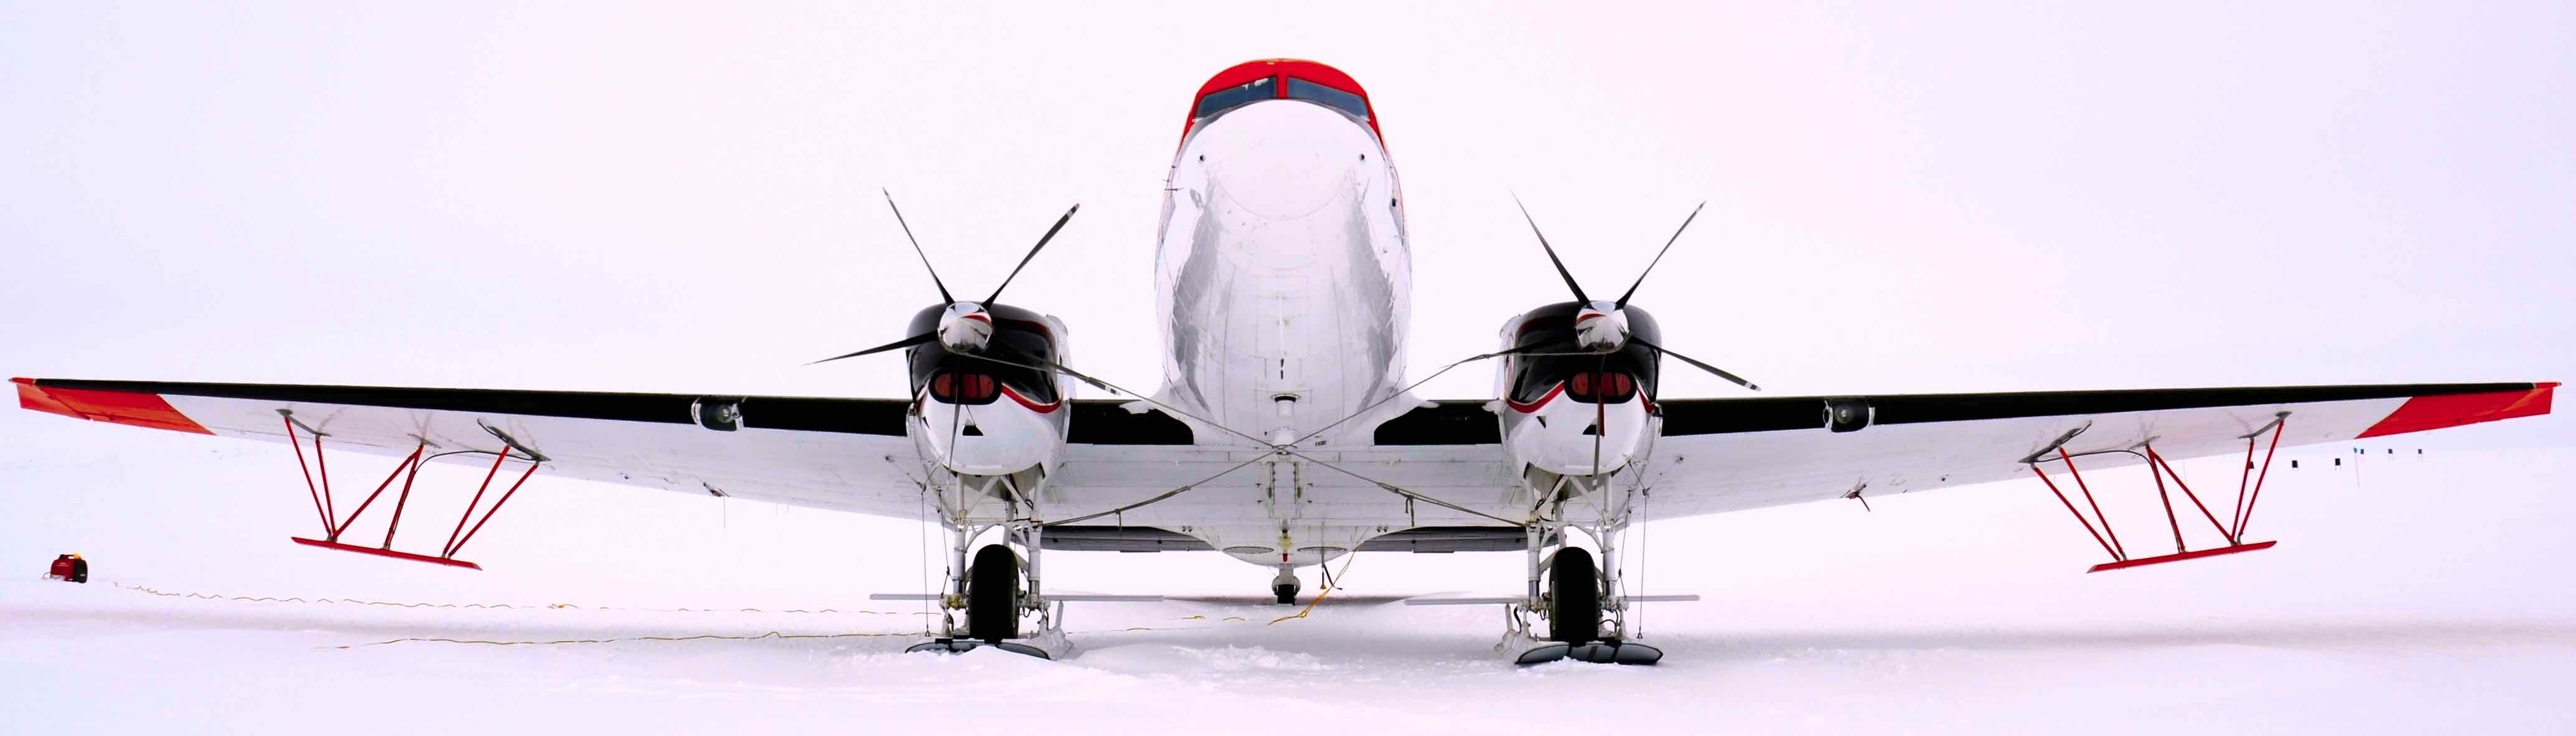
\includegraphics[width=0.95\columnwidth]{figures/JKB_chad_smaller.jpg}
\caption[]{JKB, one of the DC-3s that has been modified to carry our instrument suite. Note the antennas under the wings. (Photo: Chad Greene) \future{This figure needs a perfectly white background. DAY has a version like that.}}
\label{fig:JKB_chad}
\end{figure}

Two dipole antennas, separated by 18.95m (\figref{fig:JKB_chad}) generate the beam pattern shown in \figref{fig:beam_pattern}.
\question{I got that distance measurement from the PRIC documents. Is it also true for JKB/MKB?}
They are mounted a quarter wavelength under the wings, and both antennas are used for both transmit and receive.
\question{I'd like to add a sentence about why this mounting distance is important.}

\begin{figure}[ht!]
\centering
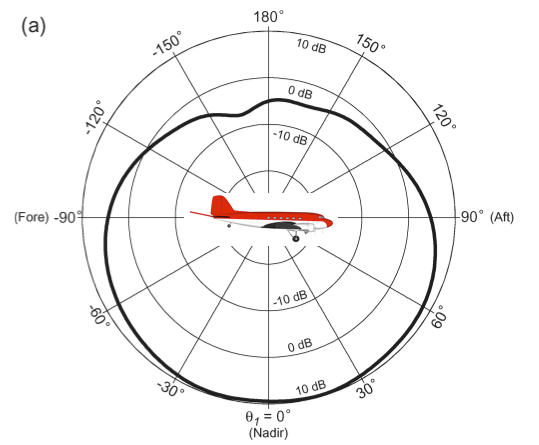
\includegraphics[width=0.48\columnwidth]{figures/beam_pattern_along_track.png}
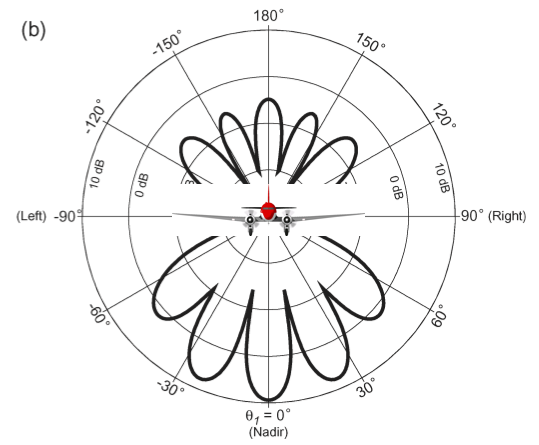
\includegraphics[width=0.48\columnwidth]{figures/beam_pattern_cross_track.png}
\caption[]{(Left) The along-track beam pattern that results from our antenna placement. (Right) The across-track beam pattern. (From \cite{Peters2007})}
\label{fig:beam_pattern}
\end{figure}

The broad beam pattern and strong side lobes mean that in addition to echoes directly below the airplane, we detect significant off-nadir energy, which adds clutter to the radargram and lowers the spatial resolution. Many of the processing steps are aimed at reducing these effects. It is easier to improve along-track resolution because we have many overlapping observations. Clutter from the sides is more difficult to reduce. 

\begin{figure}[ht!]
\centering
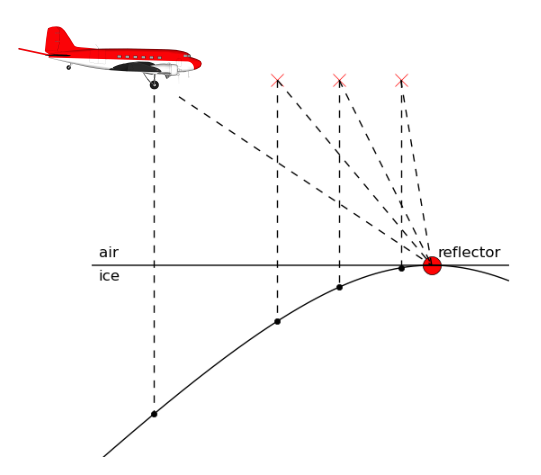
\includegraphics[width=0.5\columnwidth]{figures/hyperbola_geometry_cropped.png}
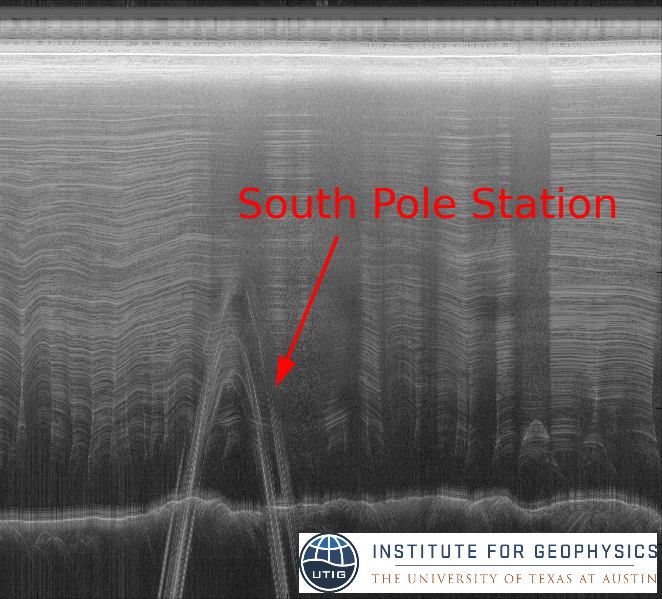
\includegraphics[width=0.48\columnwidth]{figures/NPX_SJB2_NPX02a.png}
\caption[]{(Left) geometry for strong point reflector to show up in the data as a hyperbola. (Right) Example hyperbola from South Pole Station}
\label{fig:hyperbola_geometry}
\end{figure}




\subsection{Details of Radar Electronics}
  
\future{Better block diagram of the electronics}
%\begin{figure}[h]
%\centering
%\includegraphics[width=0.4\columnwidth]{figures/GNG_block_diagram.pdf}
%\includegraphics[width=0.5\columnwidth]{figures/GNG_block_diagram2.pdf}
%\caption[]{Block diagram of radar electronics. (Credit: Gregory Ng) \todo{Better one w/ LO and only one T/R switch?}}
%\end{figure}

\future{More hardware details/specs for the PXI components and amplifier?}
The transmitted energy is a 1$\mu$s wide chirped pulse, with a 60MHz center frequency and 15MHz bandwidth. It is generated digitally by a PXI controller with samples at 200MHz, and fed into an 8kW Tomco amplifier. \figref{fig:chirp} shows the resulting transmitted pulse shape. The pulse repetition frequency of the current system is 6250Hz, which means if the airplane is flying at the nominal 90m/s, it is taking a measurement about every 1.5cm along track. \question{ADC?}

\begin{figure}[ht!]
\centering
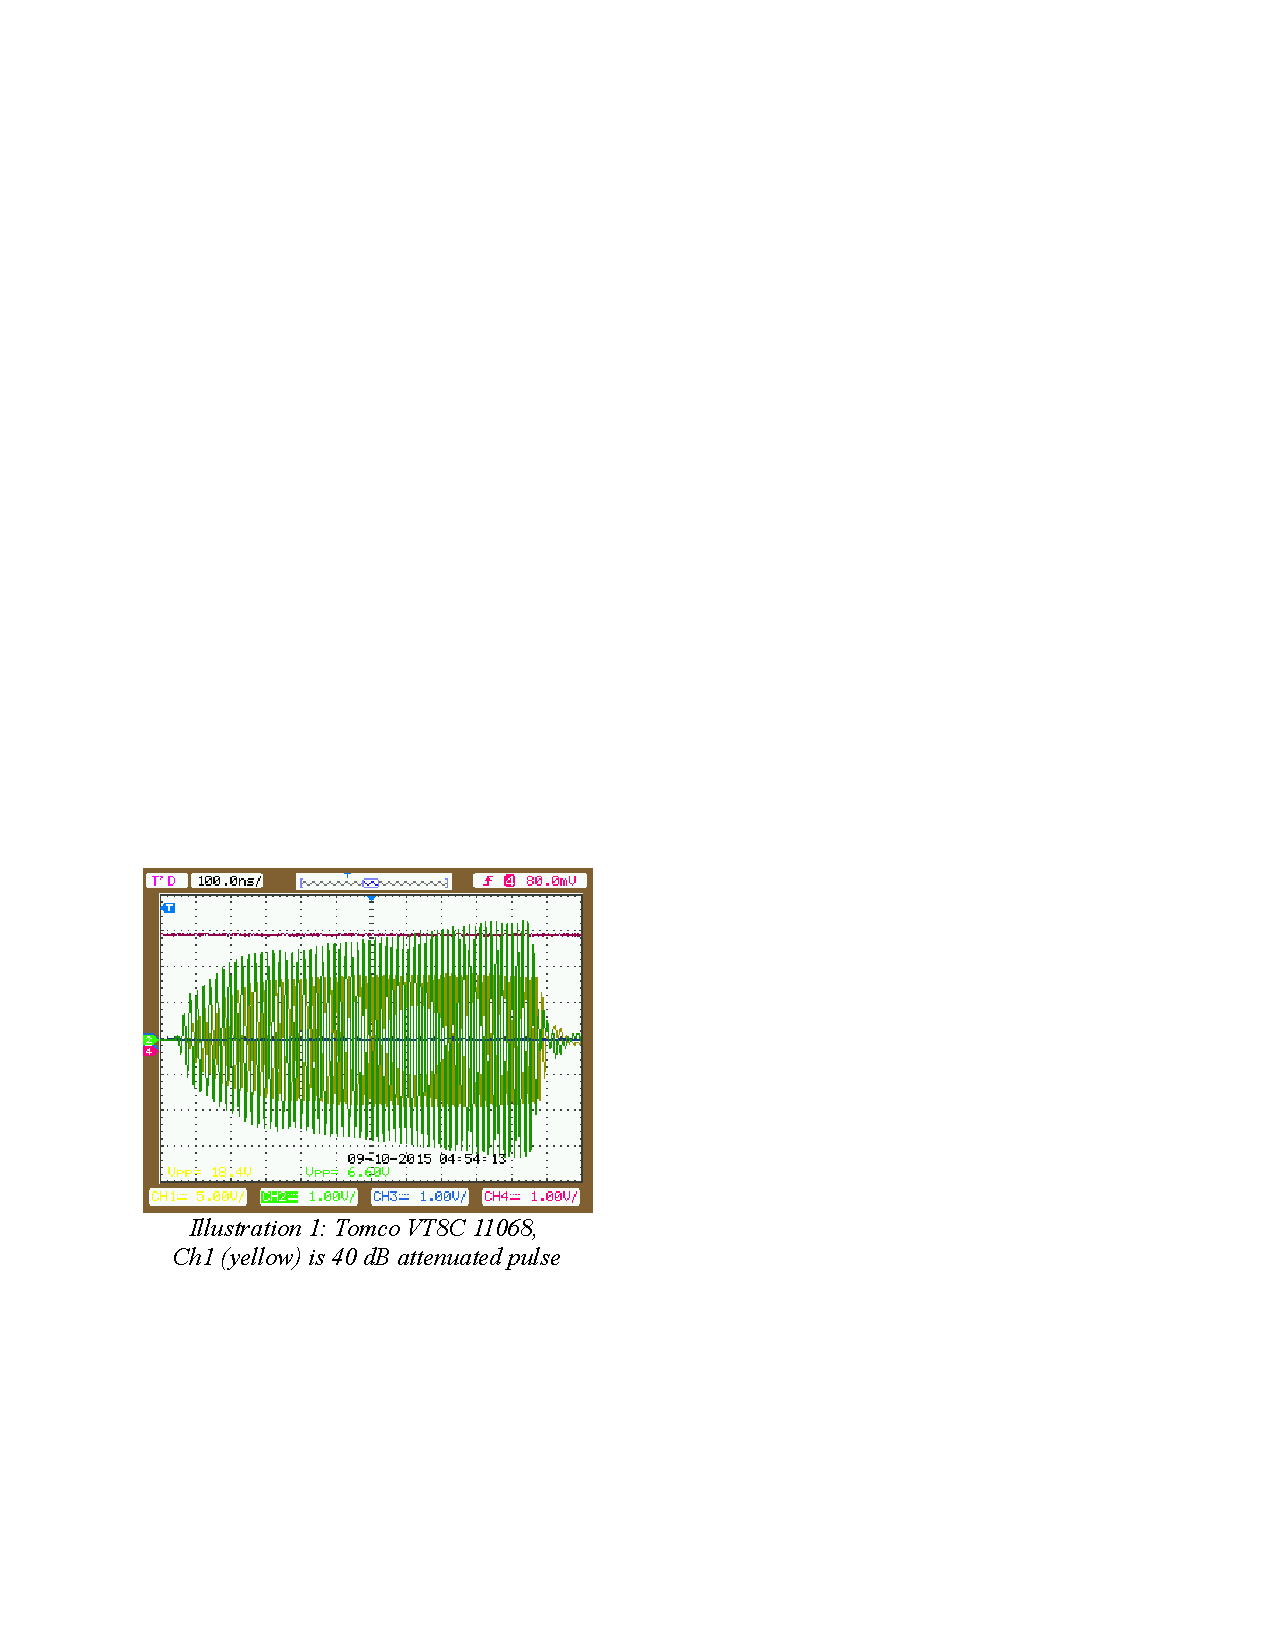
\includegraphics[width=0.45\columnwidth]{figures/tomco_pulse_shape.pdf}
\caption[]{Oscilloscope trace of attenuated amplifier output. (Credit: Gregory Ng, EC15036)}
\label{fig:chirp}
\end{figure}

As discussed in \secref{sec:beam_pattern}, we use both antennas for both transmit and receive. This is enabled by routing the amplifier's output signal through a transmit/receive (T/R) switch, a splitter/combiner, and out to the antennas. \question{more details?....}

For the system described in this report, the returned signal was downconverted before digitization. Recent improvements in digitizers has enabled us to do bandpass sampling without the downconversion. The downconversion is performed by mixing the signal with a 70MHz local oscillator, then low pass filtering the output. 

The PXI also generates a blanking signal that brackets the outgoing chirp. The receive electronics use this to determine whether to digitize the output of the T/R switches or the attenuated reference chirp from the amplifiers.

In order to achieve a 130dB dynamic range with only 14 digitizer bits, the returned signal is split into high and low gain channels. \future{ with \todo{???} and \todo{??} dB of amplification respectively.} Each channel is recorded separately; the low gain one does not saturate at the surface, so it is used for any near-surface applications, while the high gain one is used for detecting deeper layers and faint bed returns.

Before writing the data to disk, 32 consecutive traces are summed. This is required to maintain a feasible disk write rate, and the justification is the same as for software stacking in \secref{sec:coherent_stacking}. The 3 least significant bits are dropped, resulting in 2 bytes per sample.
 
% % This figure is 7-8MB total ... need to decrease that or cut it out!
%\begin{figure}[ht!]
%\centering
%\includegraphics[width=0.3\columnwidth]{figures/DSC03651_small.jpg}
%\includegraphics[width=0.3\columnwidth]{figures/DSC03649_small.jpg}
%\includegraphics[width=0.38\columnwidth]{figures/JKB_racks.jpg}
%\caption[]{(Left and Center) The electronics racks (Right) UTIG engineer Gregory Ng monitoring the radar performance during a survey flight. \todo{Better labeling of components.}}
%\end{figure}

The receiver electronics saturate at 1V peak-to-peak and write 16bits to disk (14-bit digitizer, with 32x hardware stacking and dropping the 3 least significant bits before writing to disk).
In order to to convert from counts to power or voltage we use: 

\begin{centering}
$2^{16}$ counts = 1.0$V_{pp}$ \\
$V_{rms} = \frac{1}{2\sqrt{2}}V_{pp}$ \\
0dBm = $10 \log_{10} 1mW$ \\
Power (W) = $\frac{V_{rms}^2}{Z}$ \\
\end{centering}

\future{Figure out how to format this w/ the = aligned.}
%\begin{array}
%%| c | c | \\
%$2^{16}$ counts &= 1.0$V_{pp}$ \\
%$V_{rms}$ &= $\frac{1}{2\sqrt{2}}V_{pp}$ \\
%0dBm &= $10 \log_{10} 1mW$ \\
%Power (W) &= $\frac{V_{rms}^2}{Z}$ \\
%\end{array}

%\begin{equation}
%2^{16} counts = 1.0V_{pp}, 
%V_{rms} = \frac{1}{2\sqrt{2}}V_{pp}, 
%0dBm = 10 \log_{10} 1mW, 
%Power (W) = \frac{V_{rms}^2}{Z} 
%\end{equation}

For a system with $50\Omega$) impedance, if a signal is $C$ counts peak-to-peak in the raw data it is
$10 \log_{10} \left(1000\frac{\left(\frac{1}{2\sqrt2}\frac{C}{2^{16}}\right)^2}{50\Omega}\right)$ dBm.


\question{Where does the frequency mixer fall in here? Is that accounted for in the high/low gain channel attenuation numbers? }

\subsection{Coherence}

In the context of radar, we use \emph{coherent} to mean a number of slightly different things:
\begin{enumerate}
\item To describe a radar system that is able to capture phase information about the signal. This requires sending out pulses of energy where the phase is always consistent with respect to the start of the pulse. For example, if you generated the output signal using an unsychronized oscillator and a blanking signal, you'd have an incoherent radar. It also requires sampling the returned signal at a high enough frequency and good enough precision to recover the phase information. 
\item To describe an interface that reflects energy while preserving phase. A uniform mirror-like flat surface will be coherent. If a surface is rough, reflections from different points will vary in phase, and the aggregate signal will be incoherent. 
\item To describe whether the processing applied to the data has preserved phase information. Early steps in our processing pipeline retain phase information, and later ones operate only on amplitudes. Reducing different types of noise require coherent or incoherent techniques. The ordering is important since once you've discarded phase information you can't get it back.
\end{enumerate}
    
The old radar system (grey lines in \figref{fig:all_data}) was incoherent. Adding the ability to recover the signal's phase allows us to use a chirped signal for pulse compression and perform focusing. 

%\subsection{Chirped Signal}
%
%Early ice penetrating radar systems transmitted a constant frequency pulse of energy. This meant that for a given maximum amplifier power, there was a direct tradeoff between detectability and resolution, since both were governed by the total pulse width. The longer the pulse, the more ice it could penetrate, but the lower its resolution.
%This tradeoff was eliminated by the introduction of \todo{finish this ...}
%
%\todo{Brief explanation of why we transmit a chirp rather than a constant-frequency envelope? (This is where I can cite Curlander's Ch. 3 "Matched Filters")}
%
%Our transmitted 1$\mu$s wide pulse winds up with a 3dB width of 80ns and the first nulls at 200ns\cite{Peters2007}.
%
%\question{What led to the decision to transmit a chirp, rather than some other waveform? Could we get improved characteristics by doing something else?}
%
%\question{What governs the bandwidth of the chirp? The antennas being designed }
%
%\question{Why is this hard/why didn't it get implemented until 2001? We talk about digitization/sampling rate/coherence as being the driving thing in being able to implement pulse compression. However, MUCH higher frequency applications rely on pulse compression (e.g. cell phones). How do they implement it? Is it done in analog somehow? Would this have been possible back in the day for IPR?}

\section{The \textbf{pik1} Data Product}
\label{sec:pik1}

\begin{figure}[ht!]
\centering
\includegraphics[width=1.0\columnwidth]{figures/TOT_pik1_labeled.jpg}
\caption[]{Example \textbf{pik1} data product. The numbered boxes and vertical line show regions that are used to highlight the effects of different processing steps.}
\label{fig:pik1}
\end{figure}


\textbf{pik1} is the simplest and least-processor-intensive radar data product that our group produces. It is primarily meant as a field quality control product, suitable for analyzing after each flight in order to determine whether we successfully gathered the data required to answer our scientific questions. An example can be seen in \figref{fig:pik1}. It is also used for preliminary surface and bed labeling that leads to ice thickness estimates. Our primary products meant for scientific analysis are the focused radargrams (\secref{sec:focusing}).

This rest of this section describes the processing steps involved in generating the \textbf{pik1} data product. 

\subsection{Pre-Processing Raw Data}
\label{sec:blanking}

As we transmit the signal, it also interacts with the airplane, creating a very loud noise signal that we call the \emph{main bang}. This is partially masked in hardware in order to protect the digitizers and allow us to record an unsaturated reference chirp. However, the noise continues well past the end of the hardware blanking. 

\begin{figure}[ht!]
\centering
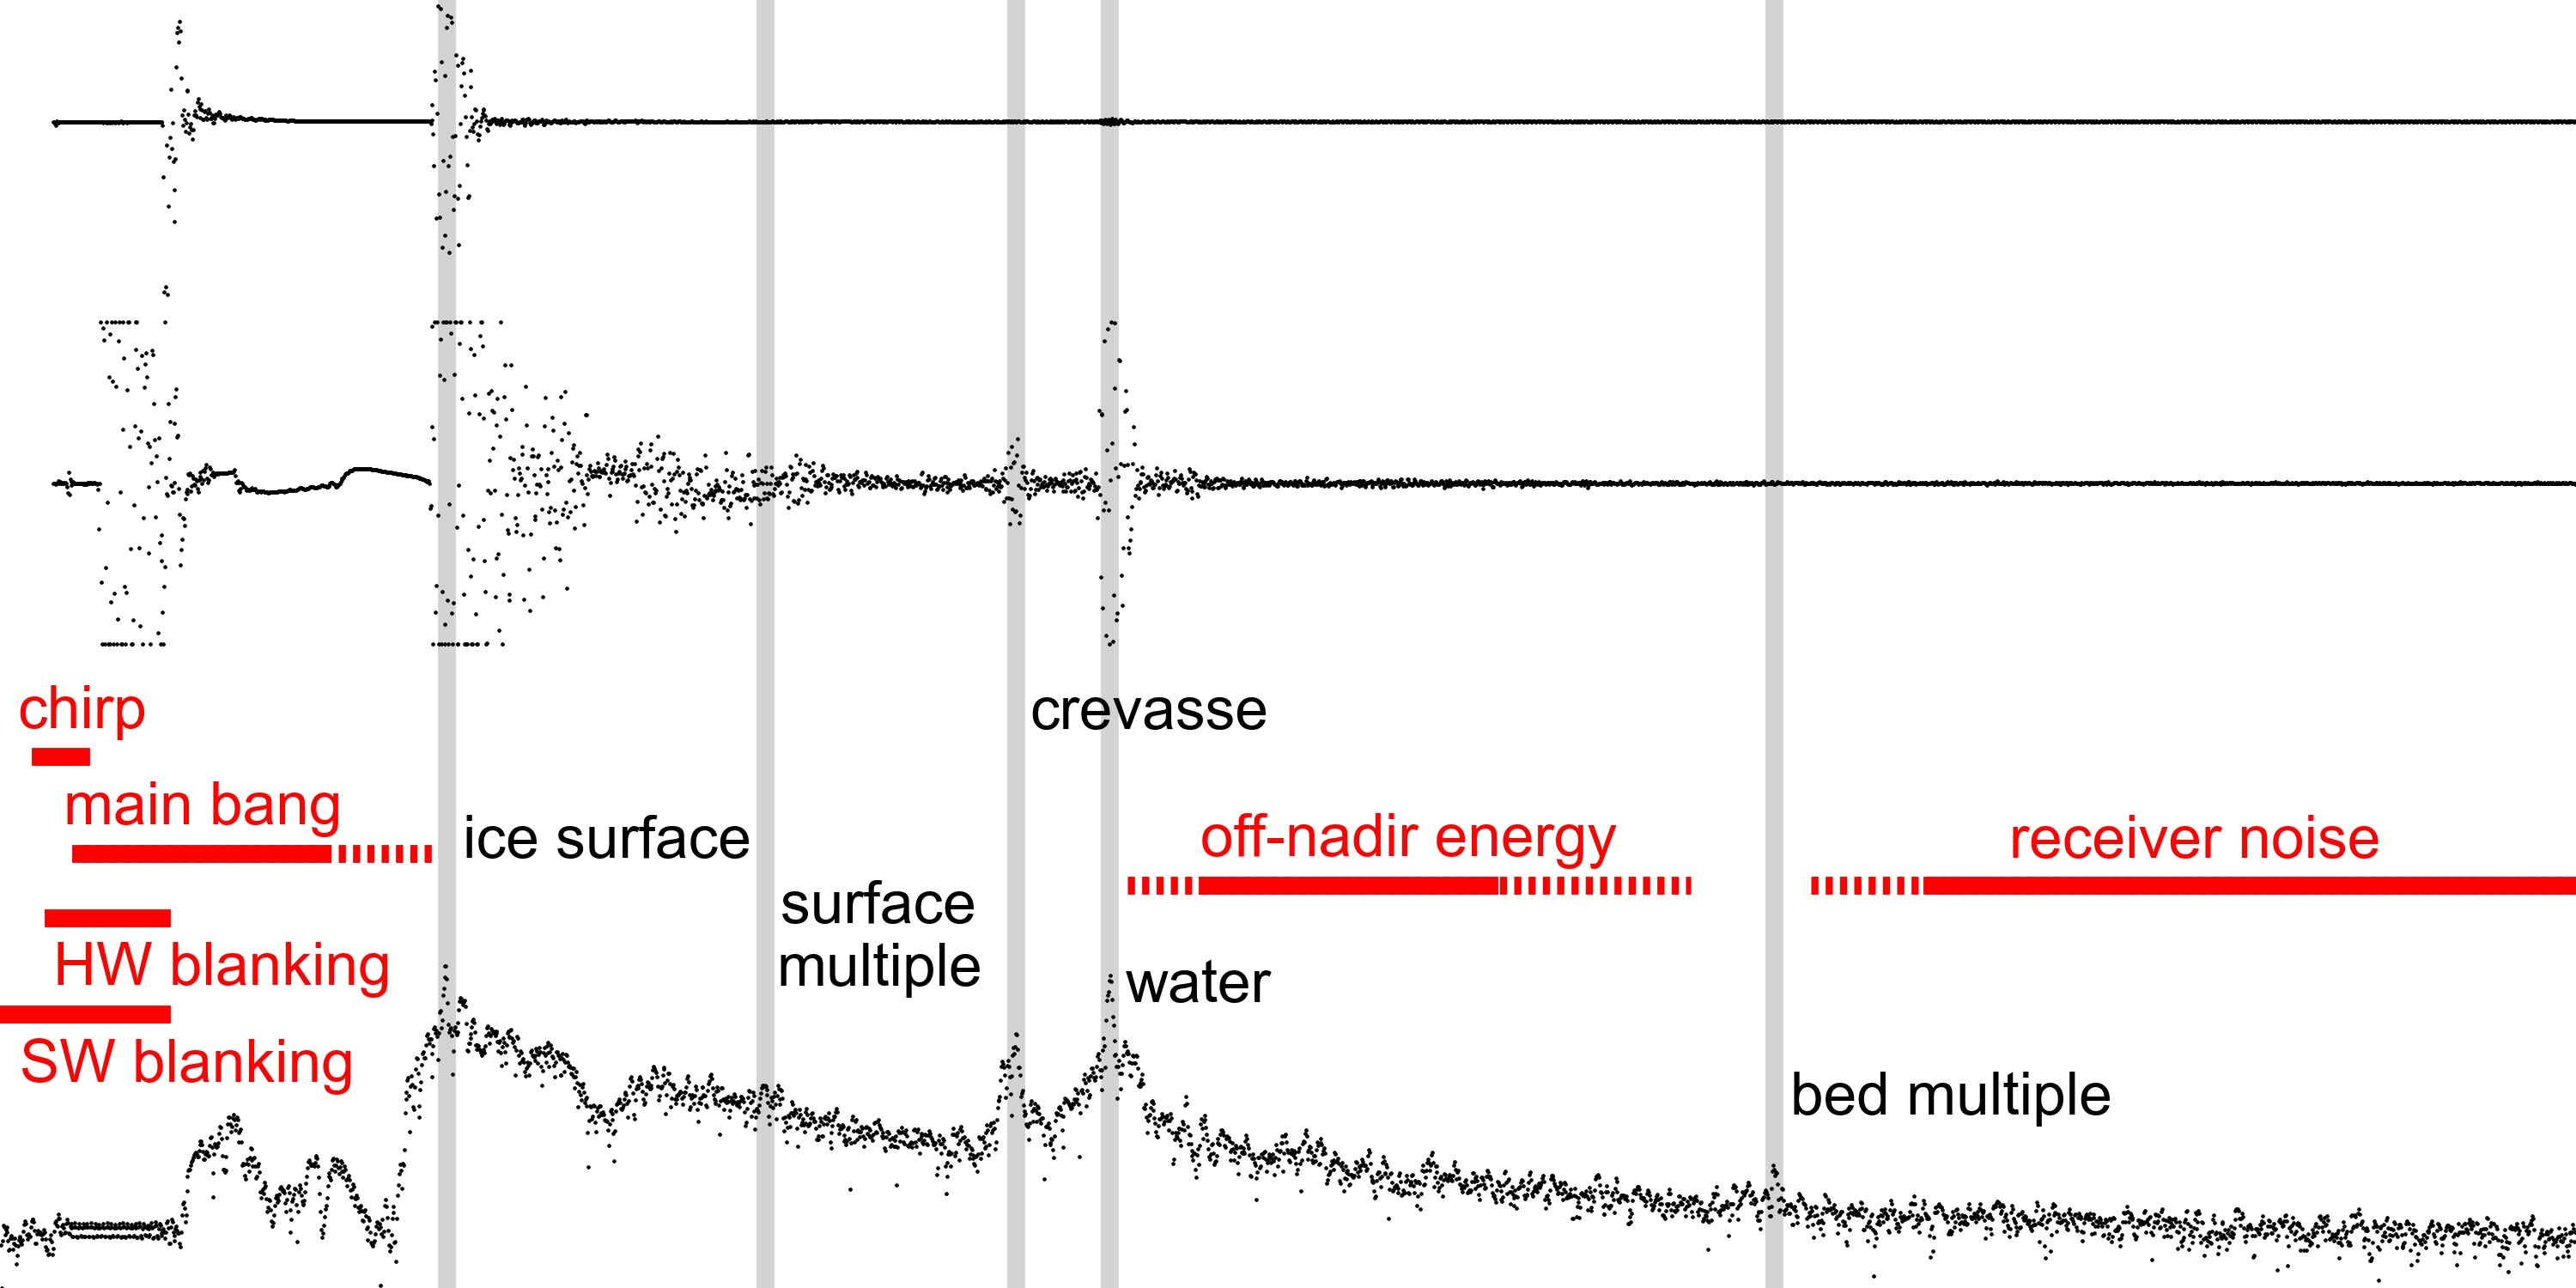
\includegraphics[width=1.0\columnwidth]{figures/trace.jpg}
\caption[]{A single raw trace as recorded by the digitizers (top - low gain, center - high gain), and the resulting textbf{pik1} product for high gain channel. (bottom). Trace location is shown as the dotted line in \figref{fig:pik1}.}
\label{fig:trace}
\end{figure}

\question{It looks like the hardware blanking isn't working correctly in the high gain channel?}

Received wisdom is that we need to blank the first $\sim$200 samples of the raw data as the first processing step in order to mask the main bang. \figref{fig:trace} shows the relative timings of the transmitted chirp, main bang, hardware and software blanking. The hardware blanking is used to switch the receiver's input from the T/R switch to an attenuated version of the transmitted pulse fed in from the amplifier's output. 

The additional software blanking step doesn't make sense to me: it was always a question of how much to blank without risking cutting off part of the surface return; the samples that are zeroed mostly overlap with the blanking that has already been performed in hardware; and I haven't found a transect where leaving this step out affects the appearance of the \textbf{pik1} product.

While the low gain channel in \figref{fig:trace} behaves as expected, the high gain channel appears to have a significant DC offset. Looking at \figref{fig:ch2_DC_artifact}, we can see that the odd dark regions under the surface only appear in the high gain data, and only where we are flying near to the surface, which suggests that these artifacts might be related. 

\begin{figure}[ht!]
\centering
\includegraphics[width=0.49\columnwidth]{figures/TOT_ch1_DC.jpg}
\includegraphics[width=0.49\columnwidth]{figures/TOT_ch2_DC.jpg} \\
\vspace{2pt}
\includegraphics[width=0.49\columnwidth]{figures/VCD_ch1_DC.jpg}
\includegraphics[width=0.49\columnwidth]{figures/VCD_ch2_DC.jpg}
\caption[]{Low gain (left) and high gain (right) radargrams from when the airplane was flying less than $\sim$600m from the surface. Transects are TOT/JKB2d/X16a (top) and VCD/JKB2g/DVD01a (bottom). The TOT data is from box \#1 in \figref{fig:pik1}.}
\label{fig:ch2_DC_artifact}
\end{figure}

The consistency of the pattern above the surface in the raw data and dechirped data suggests that it might be possible to subtract this signal out. Characterizing the noise properly would be most straightforward if I could find a transect that was flown at a very high elevation. However, it is not clear whether there is any scientific justification to doing this characterization: if it is only a near-surface effect, and only appears in the high gain data, then it's not a problem, since we can use the low gain data. However, looking at the raw data in \figref{fig:raw_radar}, it appears that the oscillations continue beyond the near surface. Thus, they might be contributing to an increased noise floor even if we can't see them in the \textbf{pik1} product. 

\future{Something about my ch1 processing is borked. Maybe the LO is a bigger deal there and it's killing my sensitivity?? I should look into it later. For now, I'm just using the data from the hierarchy in these plots.}

\future{TOT/JKB2d/X16a traces 2840-3200, samples 60-480 might be a good thing to look at for starters unless R22 has some high-off-the-deck portions... I also wonder if I can treat the signals as summations of digitizer counts}

\future{A DC offset shouldn't affect the FFT, unless it also has a frequency component...so look at its FFT as well, since something is clearly happening in the processing. I might be able to get a frequency component from looking at the stripes in \figref{raw_radar}.}


\subsection{Pulse Compression}

It is possible to see a surface and bed in the raw amplitudes recorded by the digitizer, but this image does not have anywhere near the resolution that we would hope for. 
Since we transmit a chirped signal, the first step in processing is to perform \emph{pulse compression} - also referred to as \emph{range compression} or \emph{dechirping}.
This simply requires convolving a reference chirp with each received trace, and it immediately improves the appearance of the surface and bed, as can be seen in  \figref{fig:raw_radar}.
In practice, this is done more efficiently using the convolution property of the Fourier Transform: 
$chirp \ast trace = iFFT(FFT(trace) \cdot FFT(chirp))$

\future{Reference chirp figure!}
%\begin{figure}[ht!]
%\centering
%\includegraphics[width=0.2\columnwidth]{figures/placeholder.jpg}
%\caption[]{Reference chirp used in pulse compression.}
%\label{fig:ref_chirp}
%\end{figure}

\begin{figure}[h]
\centering
\includegraphics[width=1.0\columnwidth]{figures/TOT_raw_full.jpg} \\
\vspace{2pt}
\includegraphics[width=1.0\columnwidth]{figures/TOT_dechirped_full.jpg}
\caption[]{Pulse compression sharpens interfaces. (Top) Magnitude of raw radar returns. (Bottom) After dechirping.}
\label{fig:raw_radar}
\end{figure}


Examination of \figref{fig:trace} shows that the first sample of the raw data has to be offset by 66 traces in order for it to line up with the final \textbf{pik1} data product. \future{generate exact number.} 
This is due to the fact that the reference chirp used in the pulse compression \future{, shown in \figref{fig:ref_chirp},}does not start at the first sample. 
Thus, the peak energy when convolving the reference chirp with a theoretical chirp that starts at sample 0 occurs at a later sample.\future{This needs a better explanation...something to do about the peak energy being delayed by ??? (I should be able to derive it exactly.}
\future{While I'm working on that, I should also figure out how to explain the appearance of noise in the first 50-ish samples of the pik1 trace, and why the output trace isn't perfectly zeroed by the software blanking.}

Additionally, the reference chirp must be flipped to sweep from high to low frequency. This is because the down conversion changes the signal to 70MHz - chirp, and for a 52.5~$\rightarrow$~67.5MHz chirp, this results in a 17.5~$\rightarrow$~2.5MHz signal. 


\subsection{Filtering}
\label{sec:filtering}

\begin{figure}[h!]
\centering
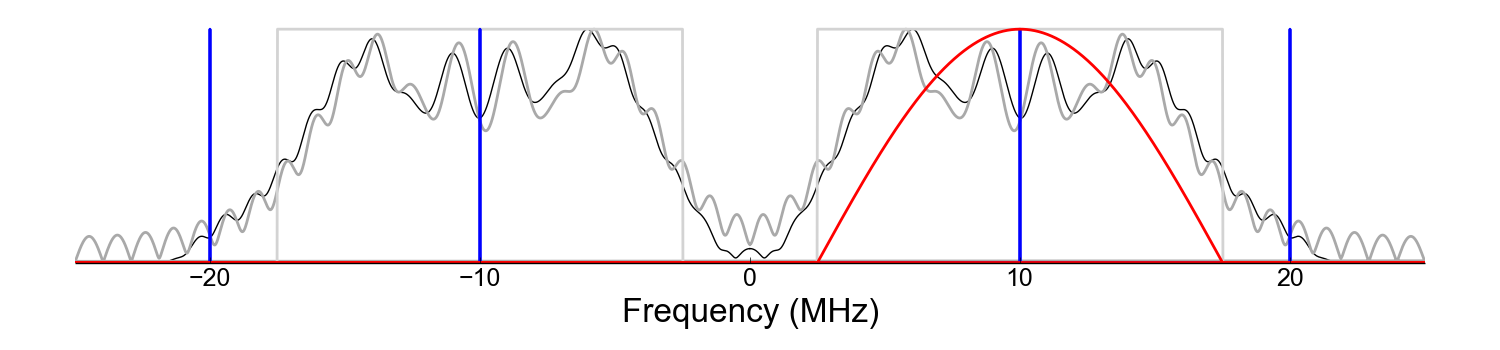
\includegraphics[width=1.0\columnwidth]{figures/filter_frequencies.png}
\caption[]{Frequency-space representation of the filter (red) and other signals in the system. FFT of Local Oscillator (70MHz) and LO's first harmonic (140MHz) are in blue. Ideal chirp frequency spectrum is light grey, 3200-bin FFT of 50MHz sampled ideal chirp in dark grey, and FFT of the chirp used in processing is black.}
\label{fig:filter_freqs}
\end{figure}

As part of the pulse compression step, we apply a window function (\figref{fig:filter_freqs}) to the trace's FFT. This has the effect of further sharpening interfaces (\figref{fig:filtered}). 

%\todo{Check that I have the "ideal" FFT correct. Is it mirrored or not?}
%\todo{See whether mirroring the hanning filter has any effect either ...}


\begin{figure}[h!]
\centering
\includegraphics[width=1.0\columnwidth]{figures/TOT_dechirped_zoom1.jpg} \\
\vspace{2pt}
\includegraphics[width=1.0\columnwidth]{figures/TOT_filtered_zoom1.jpg}
\caption[]{Zooming in on the surface shows the effect of filtering. This region is box \#2 in \figref{fig:pik1}. (Top) Dechirped. (Bottom) Dechirped and filtered.}
\label{fig:filtered}
\end{figure}

\question{I think the reason we need this is that as the range to the surface changes slightly the peak value of the convolution changes, so we need to average it out a bit? Or is it something to do with inaccuracies introduced by having to do a discrete Fourier transform rather than the continuous-time FT? I'm not sure ... I wish that I could read that chapter that Prof. Vikalo pointed out to me ...}


\subsection{Coherent Stacking}
\label{sec:coherent_stacking}

Since the data is recorded at about 195Hz (the radar pulse repetition frequency is 6250Hz; we stack 32x in hardware) and the plane flies at about 90m/s, we have traces spaced about every 50cm. 
This is excessive along track sampling for any human-viewable data product. For comparison, our across track 3dB beam width is $12^\circ$ and our along track beam width is $152^\circ$\cite{Peters2007}.
So, flying at an altitude of 600m, our effective pulse shape is 126m x 4.8km. The effective footprint is significantly smaller than this, since it is \emph{pulse limited} based the maximum off-nadir angle before returned energy begins to destructively interfere.
\future{Better pulse limited discussion; it's a bit hand-wavey here and below.}

We perform additional stacking in software; this has two primary benefits.

\future{Figure for footprint geometry!}
%\begin{figure}[ht!]
%\centering
%\includegraphics[width=0.2\columnwidth]{figures/placeholder.jpg}
%\includegraphics[width=0.2\columnwidth]{figures/placeholder.jpg}
%\includegraphics[width=0.2\columnwidth]{figures/placeholder.jpg}
%\caption[]{Left: Geometry for pulse effective footprint; Center: Geometry for surface slope; Right: Explanation for improved along-track resolution \todo{Maybe just put the math in the text?}}
%\end{figure}

First, it improves our signal-to-noise ratio. 
Since the footprints of successive pulses almost entirely overlap, we treat them as repeat measurements of the same scene, for which we'd expect the SNR to improve with $\sqrt{n}$. The maximum effective stacking depth is determined by how many consecutive returns can be added before the first and last begin to destructively interfere. (In practice, we don't want them to differ by more than $\frac{\lambda}{4}$.) This will be governed by either the \emph{pulse limited footprint} or how quickly the terrain changes. In practice, we have found that a depth of 10 works well at this stage.

\begin{figure}[ht!]
\centering
\includegraphics[width=0.48\columnwidth]{figures/TOT_filtered_zoom2.jpg}
\includegraphics[width=0.48\columnwidth]{figures/TOT_costacked_zoom2.jpg}
\caption[]{Coherent stacking improves the SNR, revealing layers. Improved horizontal resolution can also be seen at the bed. This region is box \#3 in \figref{fig:pik1}. (Left) Dechirped (Right) Dechirped and coherently stacked 50x.}
\end{figure}

\future{I need to find an example of where we can actually see the improved along-track resolution. Or is it even visible? How does it compare to the pulse-limited footprint?}

Second, it increases our along-track resolution. This technique is also referred to as \emph{unfocused Synthetic Aperture Radar} or \emph{coherent integration} \cite{Peters2005}.
The intuitive explanation of unfocused SAR is that for a single pulse, you have energy from the entire footprint given by the beam pattern. 
If you add multiple consecutive pulses, the energy from their overlapping portions will constructively interfere while the energy from the non-overlapping borders will destructively interfere. 
Thus, the more pulses you add, the smaller your effective footprint. 

\subsection{Incoherent Stacking}

\begin{figure}[ht!]
\centering
\includegraphics[width=0.48\columnwidth]{figures/TOT_costacked_zoom3.jpg}
\includegraphics[width=0.48\columnwidth]{figures/TOT_stacked_zoom3.jpg}
\caption[]{Incoherent stacking alleviates speckle. This region is box \#4 in \figref{fig:pik1}. (Left) coherently stacked 50x (Right) coherently stacked 10x, incoherently stacked 5x.}
\label{fig:incoherent_stacking}
\end{figure}

While coherently stacking the returned traces is fantastic for improving the signal to noise ratio, it is unable to address some types of noise.
\emph{Speckle} is caused by constructive and destructive interference of the waveforms. It is the same effect as you'd see looking at a laser pointer's dot. Additional coherent summation simply moves the peaks and nulls around; it is unable to eliminate them. Reducing noise due to speckle requires summing the magnitudes of the traces rather than the full waveform. We call this \emph{incoherent stacking}, and the results can be seen in \figref{fig:incoherent_stacking}.

\question{Are there other types of noise that this also helps? Looking at the figure, it also seems to make the hyperbolas clearer}



\subsection{Implementation}

Data processing pipelines that require streaming data (rather than operating on the entire data set at once) can be implemented elegantly by chaining generators in python. At the highest level, the \textbf{pik1} algorithm looks like:\\

\texttt{
\# Reads from disk and yields one trace at a time \\
traces = read\_raw\_data(...) \\
\# Gathers \emph{depth} traces and yields their sum \\
coherent\_stacks = coh\_stack\_gen(traces, depth, ...) \\
\# Performs dechirping and filtering on single input trace, yields the result \\
dechirped\_traces = dechirp\_gen(coherent\_stacks, ...) \\
\# Gathers \emph{inco\_depth} traces and yields the sum of their magnitudes \\
inco\_traces = inco\_stack\_gen(dechirped\_traces, inco\_depth, ...) \\
\# Reads one trace at a time and writes to disk \\
write\_data(inco\_traces, ...) \\
} %end texttt

\future{better pseudocode formatting?}

Since addition and convolution commute, coherent stacking and dechirping can be performed in either order. For performance reasons, we stack first. Filtering and the local oscillator correction both happen in frequency space, which means that they are performed at the same time as dechirping. The TOT/JKB2d/X16a transect used throughout this report represents just under an hour of radar data, has a raw file size of 5.8G. Generating the corresponding 111M \textbf{pik1} product required under a minute on my laptop.

\future{\question{How can I test the delay between the actual start of transmission and the first return? I assume DAY does this using LAS data s.t. LAS and RAD data agree? (But then that assumes the pitch of the plane is constant...) The timing and desired range accuracy are such that cable lengths matter.}}

\future{Add in discussion about how the pik1 processing affects the power levels / how to compute dBm from pik1 counts.}
%\subsection{Absolute Power Levels}
%
%\begin{figure}[ht!]
%\centering
%\includegraphics[width=0.2\columnwidth]{figures/placeholder.jpg}
%\caption[]{Testing the processing gain: output \textbf{pik1} counts vs. 1/2 Vpp chirp}
%\end{figure}
%\todo{Sentence about how this doesn't tell us anything about transmission losses ... I've only learned about the output of the amplifiers (I have GNG's document giving Vrms for different seasons) and what happens after the digitizer input.}
%\future{Running test chirps through pik1, see what output is. IIRC, it should be ~91dB gain?}

\future{Data Quality section!!!!!}
%\section{Data Quality}
%
%When evaluating how well an ice-penetrating radar instrument performs, key metrics include sensitivity/noise floor, vertical resolution, and horizontal resolution. \todo{Improve this ... maybe something about how we are particularly interested in this because we design our instruments in-house, so there's the potential for tight feedback between science requirements/the results of data analysis and improved hardware.}
%
%\todo{Do I want to discuss anything about resolution here? It's not what I need to know for this field season's instrument validation, and there isn't an easy way to grab it from the raw data, but it's certainly important! I'd love to wind up with a description of the factors that go into vertical and horizontal resolution ... and would be even more excited with a way to test that. }
%
%\subsection{Receiver Saturation}
%
%\begin{figure}[ht!]
%\centering
%\includegraphics[width=0.2\columnwidth]{figures/placeholder.jpg}
%\includegraphics[width=0.2\columnwidth]{figures/placeholder.jpg}
%\caption[]{Heat map of digitizer saturation for each channel.}
%\end{figure}
%
%\todo{Saturation! Discuss this. The key thing is that the surface always saturates in high gain, but we want it not to saturate in low gain, because if it does ..... I thought of a potentially-useful data product to have in the field: generate a plot of where the raw data saturates per channel. Sum up counts w/ x counts of max/min, and plot as image? Would be pretty easy to do ...)}
%
%
%\todo{Based on \figref{fig:trace}, it looks like the high gain is saturating over the ice shelf. Ugh. Mention this saturation in data quality? (especially implications for a saturated signal ... you lose vertical resolution, the ability to calculate absolute reflection coefficients, and CYG's roughness analysis doesn't work since it relies on analyzing the distribution of reflection coefficients and pulse shape.... is that correct?}
% 
%\subsection{Bandwidth}
% 
%\begin{figure}[ht!]
%\centering
%\includegraphics[width=0.2\columnwidth]{figures/placeholder.jpg}
%\caption[]{Reference chirp - want to make sure we have sufficient bandwidth}
%\end{figure}
%
%Vertical resolution is primarily controlled by the bandwidth of the transmitted chirp.
%\todo{For the reference chirp, how do we check bandwidth? Check that it's not saturated, and then convolve it with itself and find width of peak? => Look at GNG's example code ex-chirpqc.py}
%
%\subsection{Dynamic Range and Noise Floor}
%
%\begin{figure}[ht!]
%\centering
%\includegraphics[width=0.2\columnwidth]{figures/placeholder.jpg}
%\caption[]{Hockeystick plot - By looking at low gain vs high gain return strengths we can determine if we are saturating where expected and what our noise floor is}
%\label{fig:hockeystick}
%\end{figure}
%
%We are interested in detecting weak bed echoes from under more than 4 kilometers of ice. We also need to be able to accurately detect the ice surface. This leads to a spec that we expect our system to detect echoes with input power at the digitizer of -120dBm and to not saturate at 4dBm. 
%
%This can be tested by plotting the power of returns from the high and low gain channels against each other, as in \figref{fig:hockeystick}. 
%
%\todo{Discuss how to interpret the plot ... saturation at high values, hitting the noise floor at low values.}
%
%\todo{I think that the hockeystick plot on the raw data might tell us about the digitizers themselves (esp if we assume that it's zero-mean), but it won't tell us about system sensitivity. If we do it on every pik1 trace/sample, that'll tell us about the stacked data. Doing it on only picked data would give us a sense of what has actually been recovered.}
%
%\todo{Theory of digitizers and quantization error: Dusty, week2, Digitizers.pdf (Synthetic Aperture Radar by John Curlander and Robert McDonough)}
%
%\begin{figure}[ht!]
%\centering
%\includegraphics[width=0.2\columnwidth]{figures/placeholder.jpg}
%\caption[]{Noise floor - plot single trace, like DAY's QC plots, coherently stacked 0,2,4,8,16,32,64x to show converging to expected minimum (which will be dB below max echo - remember to divide by \# of times stacked to get correct reflection coefficients.)}
%\end{figure}
%
%
%\todo{This figure should have a zoomed-in background of the high gain pik1 data product (over an area of interest) with the location of the trace dash-dotted, then [1,2,5,10,25,50,100,200,1000] traces averaged plotted in a range of colors (blue to red?). Then plot saturation and theoretical noise bounds. (I'm not sure what they are ...)
%X16a trace 3880 is a good one; show 3700-4200 and samples 400-3200. colorscale will depend on final product ... }

\section{Local Oscillator Noise}

Some energy from the 70MHz local oscillator signal used in the frequency down conversion leaks through the low pass filter. When there is very little energy coming back from the antennas, this signal can become significant. \figref{fig:LO_stripes} shows horizontal stripes that result from this signal. 
(Of course, the stripes that are visible when the full radargram is shrunk down for plotting are aliased from the actual frequency.)

\begin{figure}[ht!]
\centering
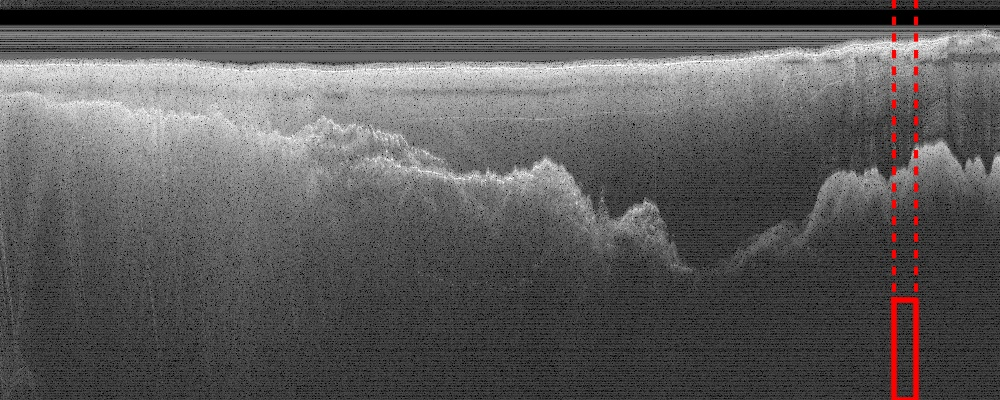
\includegraphics[width=0.89\columnwidth]{figures/TOT_LO_stripes_d.jpg}
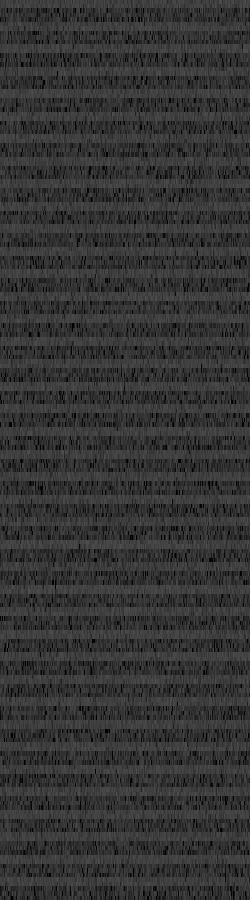
\includegraphics[width=0.099\columnwidth]{figures/TOT_LO_stripes_zoom.jpg}
\caption[]{(Left) Data product with horizontal stripes due to aliased signal leakage from the 70MHz local oscillator. Rectangle shows automatically-selected quiet region for LO noise characterization. (Right) zoomed in on last 200 samples.}
\label{fig:LO_stripes}
\end{figure}

In addition to being a visual distraction, the energy leakage that causes these horizontal stripes also contributes to a higher noise floor. Since the noise floor is a key performance metric of our system, several people had previously tried to come up with a processing improvement that would reject this LO noise. 

When I started looking at \textbf{pik1}, the existing way of dealing with this noise was to modify the FFT of the returned trace by replacing the values of the 4 bins contaminated by the LO noise with the average of their neighbors. This seemed to work (it fixed the noise floor issue) but whenever there were bright bed reflections it introduced the vertical streak artifacts that are apparent in \figref{fig:example_data}.

%\begin{figure}[ht!]
%\centering
%\includegraphics[width=0.49\columnwidth]{figures/TOT_quiet_region.jpg}
%\includegraphics[width=0.49\columnwidth]{figures/VCD_quiet_region.jpg}
%%\includegraphics[width=0.2\columnwidth]{figures/placeholder.jpg} % I'm missing the THW data to produce this plot :-(
%\caption[]{Rectangles show automatically-selected quiet region for LO noise characterization. (Left) TOT/JKB2d/X16a (Right) VCD/JKB2g/DRP01a. \todo{VCD is a bad selection - it grabbed the region w/ no data. This plot could just as well be done with the LO noise figure...}}
%%  and  THW/SJB2/DRP02a(200?), 
%\label{fig:quiet_regions}
%\end{figure}

\begin{figure}[ht!]
\centering
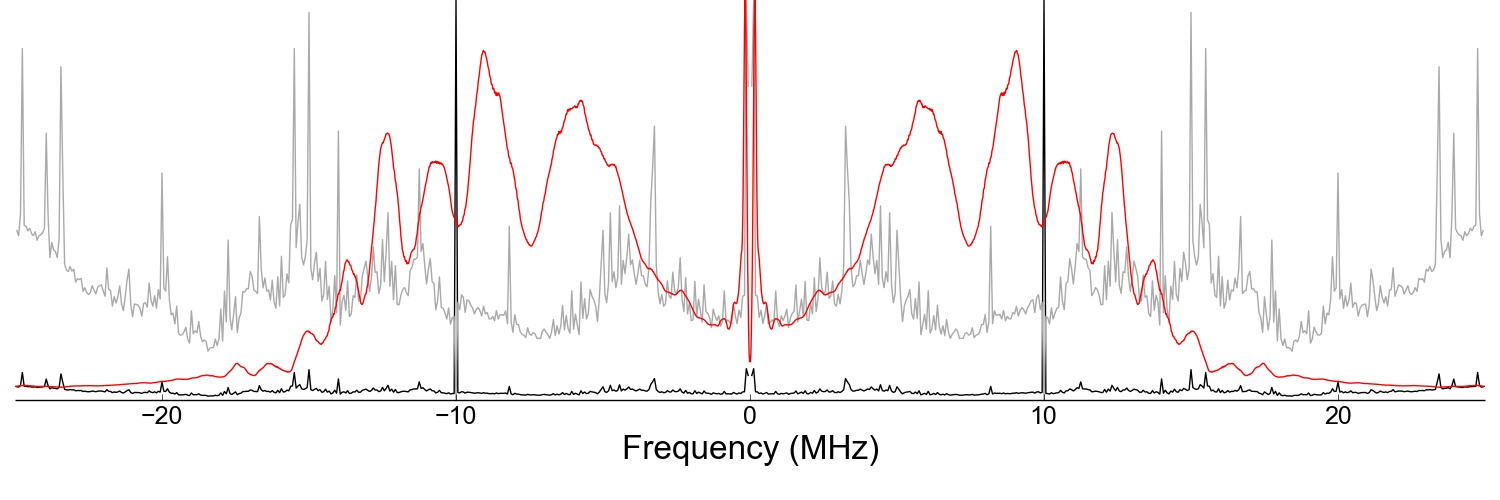
\includegraphics[width=1.0\columnwidth]{figures/LO_fft.jpg}
\caption[]{Frequency analysis TOT/JKB2d/X16a's selected quiet region as shown in \figref{fig:LO_stripes}. Red is average of the FFT of full traces in the region between the dashed lines. Black is (normalized) FFT of the selected region within the box, with the value at 0MHz removed. Grey is (normalized) FFT of the selected region with the components at 0, 10 and -10MHz removed. Vertical scale is linear.}
\label{fig:LO_fft}
\end{figure}

An obvious approach to removing this noise would be to find a region of the transect with minimal echo signal energy and characterize its frequency content. Supposedly a similar approach had been tried before; I do not know why they were unable to get it to work.
There are a few subtleties to this approach.

First, looking at \figref{fig:LO_fft}, it is clear that the LO's contribution cannot be isolated if we take the FFT of full traces (red). However, but if we limit ourselves to the last 800 samples, we obtain clear peaks at -10 and 10Mhz (black). After removing those peaks, there are no additional dominant noise frequencies (grey). Due to the filtering discussed in \secref{sec:filtering}, only the peak at 10MHz is relevant. Thus, to get rid of the LO noise we can simply subtract off the magnitude and phase of the 10MHz bin from the data's FFT. 

The quiet region must be chosen such that the phases will match up between region and the full transect. Using traces 2400-3200 has the nice property that the phase of a 10MHz signal will be the same as for traces 0-3200. Using a different subset of traces would require adjusting the computed noise phase.

Converting the noise amplitude and phase determined from a 800-point FFT to values that can be used with the 3200-point FFT given by: $FFT_{3200}[4k]=4FFT_{800}[k]$, where the factor of 4 is from 3200/800.

Finally, care must be taken to properly scale the correction based on how many traces were used to calculate it and how many traces have been stacked before it will be applied.

The phases vary between transects, and we have thousands of transects, so implementation of this correction will be made significantly easier if we automatically choose a quiet region. This automatic selection has been implemented and shown to work on a few transects. QC images such as \figref{fig:LO_stripes} can be generated showing which regions were selected. In the case of a transect that consists entirely of deep ice where a sufficiently quiet region cannot be found, I can think of two alternatives. The first alternative would be to use fewer than 800 samples; the only real constraints are that more samples are better, the number of samples used needs to evenly divide 3200 (for cleanly converting between FFTs with different numbers of bins) and needs to be a multiple of 5. It might also be possible to extend into using the last 237 traces that are normally discarded in order to keep our current system's data consistent with previous data.

%\begin{figure}[ht!]
%\centering
%\includegraphics[width=0.2\columnwidth]{figures/placeholder.jpg}
%\includegraphics[width=0.2\columnwidth]{figures/placeholder.jpg}
%\includegraphics[width=0.2\columnwidth]{figures/placeholder.jpg}
%\caption[]{Hockeystick plots for cinterp, w/, w/o LO correction on X16a. The hope is that this shows the improved dynamic range.}
%\end{figure}

\future{Discuss how we tested the correction by looking at the hockeystick plots. This will also help to validate their usage for detecting system performance, since we know that w/o the LO correction the background noise should be higher.}

\future{I may also need to do a noise floor figure to show the difference. Rather than the background image, I'd just do the different traces, with the 3 diff systems in different colors. I may need to do different saturation for the diff stacking depths? Or can I even do this post-correction? ... I'd be stacking after the FFT, but that's fine.}


\begin{figure}[]
\centering
\vspace{-30pt}
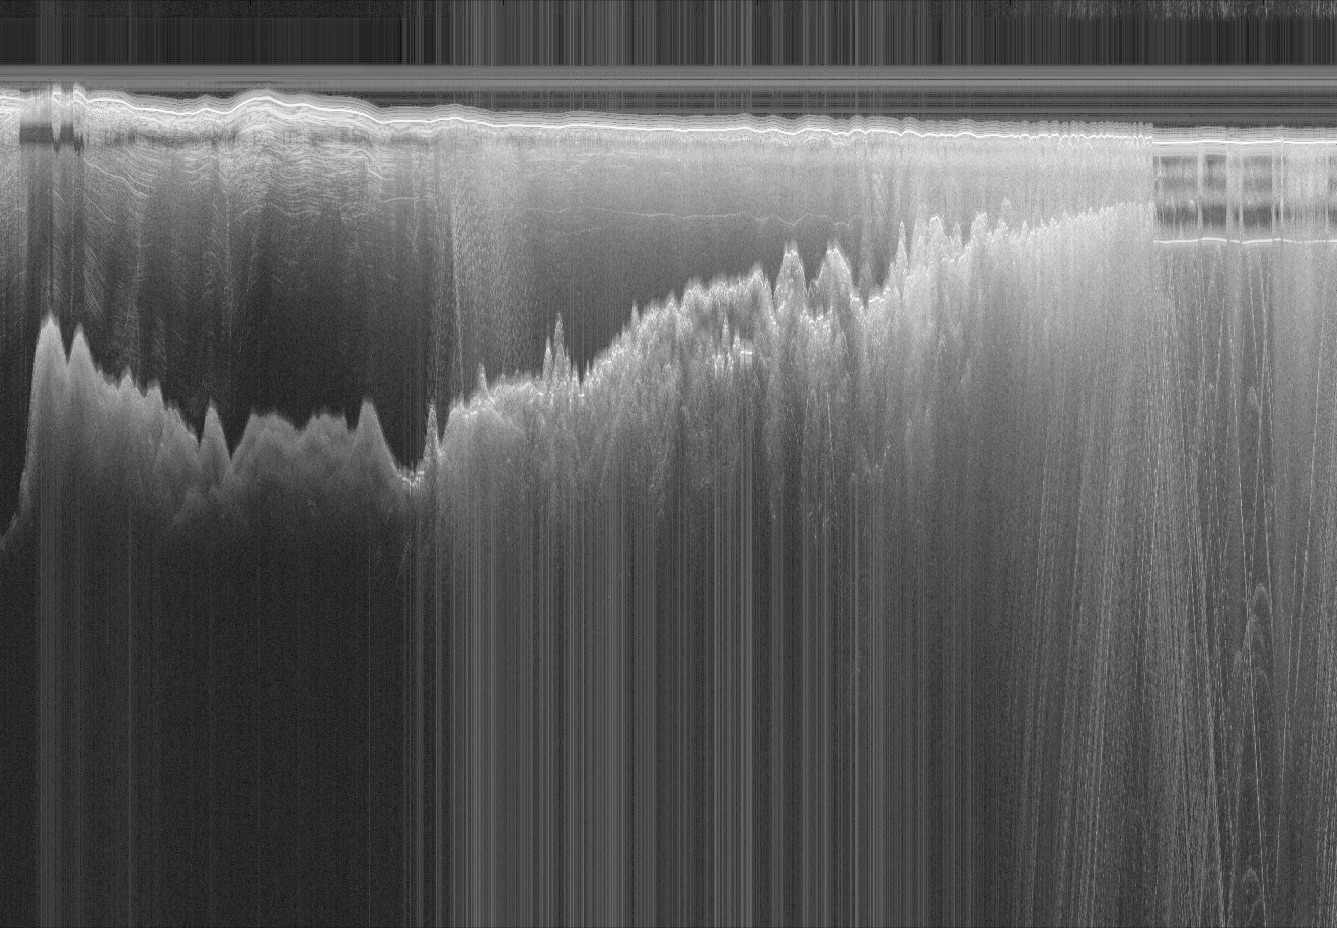
\includegraphics[width=0.495\columnwidth]{figures/TOT_X14d_old.png}
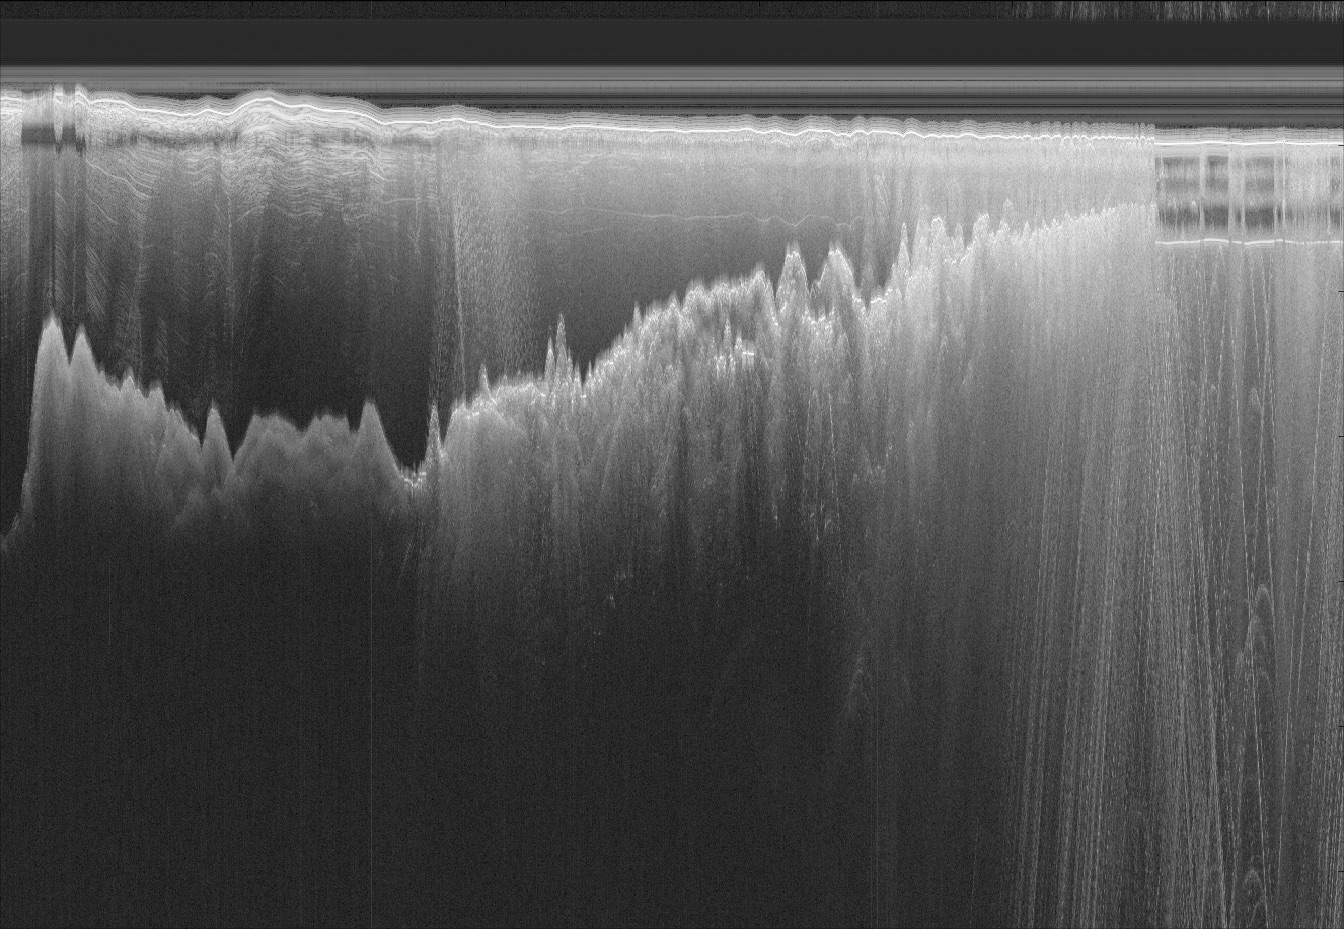
\includegraphics[width=0.495\columnwidth]{figures/TOT_X14d_new.png} \\
\vspace{2pt}
\includegraphics[width=0.495\columnwidth]{figures/TOT_X16a_old.jpg}
\includegraphics[width=0.495\columnwidth]{figures/TOT_X16a_new.jpg} \\
\vspace{2pt}
\includegraphics[width=0.495\columnwidth]{figures/THW_old.png}
\includegraphics[width=0.495\columnwidth]{figures/THW_new.png} \\
\vspace{2pt}
\includegraphics[width=0.495\columnwidth]{figures/VCD_old.png}
\includegraphics[width=0.495\columnwidth]{figures/VCD_new.png}
\caption[]{Demonstration of \textbf{pik1} improvements showing old (left column) and new (right column) approaches to LO correction for transects significantly affected by LO noise.}
\label{fig:LO_results}
\end{figure}

\section{Discussion}


The local oscillator correction does not only apply to the \textbf{pik1} data product described in \secref{sec:pik1}: it impacts every data product that we generate from the affected seasons' data. Improved digitizer performance has allowed the newest version of the receiver electronics to perform bandpass sampling and eliminate the LO, so this will not be needed for last season (dark grey lines in \figref{fig:all_data}'s map) and any future seasons.

\future{Does this also impact reflection coefficients? I wonder if they're less noisy with the new processing ... it would be good to do a plot like the hockey-stick plot for the available picks.}

\figref{fig:LO_results} shows the improvement in \textbf{pik1} for 4 problematic transects. From top to bottom, they are: TOT/JKB2d/X14d (2010/2011), TOT/JKB2d/X16a (2010/2011), THW/SJB2/DRP02a (2004/2005), VCD/JKB2g/DVD01a (2011/2012). 
The elimination of the vertical stripes has made it possible to identify what we call \emph{basal multiples} in some ice shelves. These are echoes corresponding to the radar energy that reflects from the ice/air interface and makes two round trips through the ice shelf. 

\begin{figure}[ht!]
\centering
\includegraphics[width=1.0\columnwidth]{figures/TOT_multiples.jpg}
\caption[]{Image showing surface (two round trips between plane and ice surface) and basal (two round trips between air/ice and ice/water interfaces) multiples under an ice shelf.}
\label{fig:multiples}
\end{figure}

\figref{fig:multiples} shows some of the basal multiples that were not apparent in the old \textbf{pik1} product. These are valuable for a number of reasons. First, interpreting radar data over ice shelves is very challenging. Due to the presence of basal crevasses, it can be hard to tell which echo actually corresponds to the ice-water interface and leads to an accurate ice thickness calculation. If the multiples are present, it is almost certain that they correspond to a reflection off basal interface and not a crevasse. Second, they can be used to improve inferences about the melt/freeze distribution of the ice shelf.

The radar equation gives the received power ($P_r$) as a function of radar system parameters and the properties of the media that the signal has traveled through:
\begin{equation}
P_r = P_t \left(\frac{\lambda}{4\pi}\right)^2 \frac{G_a^2 T^2 L_i^2 L_s G_p}{\left[2\left(h+z/n_2 \right) \right]^2}R
\end{equation}
The radar instrument is characterized by its transmitted power $P_t$, center frequency wavelength in air $\lambda$, antenna gain $G_a$ and system losses $L_s$. The spreading loss $\left[2\left(h+z/n_2 \right) \right]^2$ depends on the ice thickness $z$, airplane height above the ice surface $h$ and the ice's index of refraction is $n_2=1.78$. $T$ is the one-way transmission loss for the air/ice interface. 

The radar signal attenuates due to dielectric loss as it passes through the ice, represented by $L_i$, and the basal reflection coefficient $R$ varies depending on the characteristics of the bed. Ice loss is predominantly controlled by temperature, while the reflection coefficient depends on both basal roughness (scattering losses can be $\sim$10dB) and whether there is water at the bed, which creates a much stronger reflection.

Usually, a dielectric loss model is assumed and the radar equation is used to solve for $R$ in an attempt to identify water at the bed. However, if you know what the basal properties are, it can also be used to invert for $L_i$ and thus ice temperature. 
In the context of an ice shelf, this is reasonable - we know that there is water at the base, and there are specular regions where we can assume minimal scattering. 

Having the multiples is particularly valuable because if we have $P_r$ from the primary ice/water echo and the multiple, all of the terms other than $L_i$ and $R$ cancel out, reducing the uncertainty in the resulting calculations. 
The temperature of an ice shelf is interesting because it will give us information about the melt and freeze distribution: melt will locally depress the column-average temperature, leading to higher reflection coefficients. I hope to use this technique to test hypotheses about how channels in the shelf affect melting.
\future{I need lots of science references here!}
\future{\question{What's the balance between melt/freeze affecting temperatures and advection moving the record around?}}


\section{Future Work}

\subsection{Raw Radar Data and \textbf{pik1}}

While I have spent significant time looking into the \textbf{pik1} data product, I still have some questions that I'd like to investigate further:
\begin{itemize}
\item Why do we use the reference chirp that we use, and where did it come from? It doesn't match the theoretical chirp or the reference recorded from the amplifier's output. \future{Is this true? I haven't actually plotted the recorded reference chirp.} The goal is to match the output pulse shape as transmitted from the antennas, but we are not able to directly measure that. In the past, Duncan Young has attempted to use the received signal from sea water (since it is a fantastic reflector), but he says that it wound up being a good sea water detector but not good for other applications.
\item I'd like to dig into the high gain channel DC noise as discussed in \secref{sec:blanking}.
\item \secref{sec:filtering} visualized the effects of filtering as currently implemented, but I still don't properly understand why that's the right thing to do in this application.
\item I would like to perform a quantitative analysis of which stacking depth is ideal, since at this point all I have is the qualitative fact that the \textbf{pik1} product is an improvement over no stacking. This is the investigation that's least likely to make it into my group's released data products due to an issue with data consistency. We could change the balance between incoherent and coherent, but all of our final data products have the same horizontal resolution, corresponding to a total stack depth of 50x. \future{Maybe I should also do a figure showing different stacking depth choices on the image, in addition to the planned single-trace noise floor one?}
\end{itemize}

\future{I want to understand more about the dark bands below the surface: I think there are two different effects that we're observing in this transect. I'd be willing to believe that one of them is the beam pattern (represented in the first 80\% of the transect), but the part at the end looks different - in the raw data, it matches up with the main bang, so it might be some interference there? It also seems to match up with the surface looking really funny - does it saturate? Or are we turning s.t. it's much weaker? Or something else?}

\subsection{Focusing}
\label{sec:focusing}

\begin{figure}[ht!]
\centering
\includegraphics[width=0.325\columnwidth]{figures/DAY_pik1.pdf}
\includegraphics[width=0.325\columnwidth]{figures/DAY_foc1.pdf}
\includegraphics[width=0.325\columnwidth]{figures/DAY_foc2.pdf}
\caption[]{Image showing \textbf{pik1}, \textbf{foc1}, \textbf{foc2} for the same region of a transect. Note the improved layer resolution. (Credit: Duncan Young)}
\end{figure}
\future{I'd also like an example of it improving the ice shelf basal picking!}

Our group's main radar product is \emph{focused} radar data. Focusing uses the fact that as the plane flies a point reflector will show up as a hyperbola in order to ``move'' the energy that creates the hyperbola tails shown in \figref{fig:hyperbola_geometry} back to the point that generated it. The resulting image is often much less cluttered, allowing better identification of the bed reflection and internal layers. It does this by convolving a reference function with the raw radargram. This is a very computationally expensive operation because that reference function is a 2D array that must be computed for every different combination of point depths below the surface and plane height above the ice. 

We generate two different focused products, \textbf{foc1} and \textbf{foc2}, corresponding to different widths of the reference function.
Comparing the results of different focusing lengths is used in generating estimates of specularity \cite{Schroeder2015}.

\question{I don't understand how the doppler frequency fits into focusing. ...and doppler comes up in the requirements/traceability matrix, and in a lot of discussions.}

\future{Over-focusing example!}
%\begin{figure}[ht!]
%\centering
%\includegraphics[width=0.2\columnwidth]{figures/placeholder.jpg}
%\caption[]{show over-focusing on ice shelf}
%\end{figure}

On ice-shelves, it is known that focusing doesn't work very well. This is because the algorithm assumes that all reflectors are point sources generating hyperbolas. However, there are often basal crevasses, which are fantastic corner reflectors (which send the returned energy back on a vector parallel to the incident vector.) If the crevasse is aligned obliquely to the flight path, the hyperbola will have a different curvature than you'd expect for one generated by a point source at the hyperbola's apex. \future{as shown in \figref{fig:crevasse_geometry}.}

I am interested in whether we can use this difference in hyperbola geometry to determine the angle that the crevasses are aligned to the flight path. Ideally, this would be done automatically; I wonder whether it is possible to calculate a set of focused radargrams assuming different crevasse orientations, and use the relative intensities in each radargram to determine the most likely orientation. While I understand the intuition of focusing, I have not yet had the chance to look into any implementation details, so I don't have a very clear idea of what is computationally feasible. The alternative is to hand-label crevasse tails and fit a curve to them, but this requires a lot of human effort and would only work for very well defined hyperbola tails, limiting where it is applicable.



\future{Crevasse geometry figure!}
%\begin{figure}[ht!]
%\centering
%\includegraphics[width=0.2\columnwidth]{figures/placeholder.jpg}
%\caption[]{Graphic showing the geometry of a crevasse's hyperbola.}
%\label{fig:crevasse_geometry}
%\end{figure}

\future{\todo{For \figref{fig:crevasse_geometry}, I'm picturing a plan view showing the reflection point as the plane flies, then a vertical section showing the expected crevasse shapes as a function of orientation angle. I should also compute the different shapes as a function of cross-track distance of a point reflector for completeness...both on the surface and through the ice. Proper discussion of using this in focusing would require me better understanding how focusing is actually done, and whether there's any chance in hell of inverting for most probable reflector geometry. Ooooh ... for looking for crevasses, it might be enough to convolve the expected hyperbola for a given angle, and see where on the image lights up? (Is there any need to normalize for actual brightness if I really want a heat-map of where stuff is off to the side? Also, would you use a kernel that matches the expected brightness, or one that inverts for it somehow?) Is focusing really just a 2D FFT over a moving window?}}

\future{This would be a really fun thing to do - maybe I can use MIS and Amery data if we fly over that crevasse field? I don't trust the ELF, so ask JSG to get pictures out the window of the alignment w/r/t the flight path.}


\subsection{Multi-Antenna Processing}

An emerging area of research is using multiple receive antennas to enable beam forming.
While the sparse nature of the flight lines and expense of collecting data in Antarctica mean that the maps will still be interpolated from 1-D flight lines, it is important to be able to determine which direction energy returned from in order to reject clutter when attempting to identify the ice/bed boundary.
Recall from \secref{sec:beam_pattern} that the radar's beam pattern has relatively strong side lobes at $\sim23^\circ$ off-nadir.
This means that we will often receive echoes that appear to be a bed reflection but are actually from off to the side. 
The radargrams in Figures \ref{fig:off_nadir_mountains} \& \ref{fig:off_nadir_ice_shelf} illustrate this problem.

\begin{figure}[ht!]
\centering
\includegraphics[width=0.6\columnwidth]{figures/MIS_JKB2e_Y25a_full.png}
\includegraphics[width=0.3\columnwidth]{figures/MIS_JKB2e_Y25a_0.png}
\caption[]{(Left) Radargram taken along the edge of the ice shelf where the echo from the side of the shelf could be mistaken for a bed reflection if the interpreter wasn't careful. (Right) Flight path for the radargram. Ice shelves are blue, open water is grey. Note how the geometry matches with the radargram.}
\label{fig:off_nadir_ice_shelf}
\end{figure}

\begin{figure}[ht!]
\centering
\includegraphics[width=0.8\columnwidth]{figures/ICP2_JKB1a_F09T01a_full.png}
\caption[]{Radar data from flying down a valley. There is significant clutter from the mountains to either side.}
\label{fig:off_nadir_mountains}
\end{figure}

Last season, UTIG fielded a system called MARFA that independently records from each of two antennas. 
This means that the phase difference between the two antennas can be used to determine whether an echo originates from directly below the airplane or from off to the side.
This has been demonstrated to successfully discriminate surface clutter \cite{Castelletti2015}.
Unfortunately, this is only two antennas, and they have a wide enough baseline that phase cycles relatively rapidly. 
We are working on how to visualize the phase information, and how to extend this result to basal clutter.

CReSIS has been experimenting with recording from multiple antennas oriented across track with their MCoRDS radar instrument.
They have also succeeded at clutter discrimination \cite{Gogineni2014}, and have managed 3D swath surface and bed reconstructions \cite{Wu2011}.

\section*{Acknowledgements}
I owe a huge thanks to my colleagues at UTIG for our discussions about this radar system. 
Duncan Young, Gregory Ng and Scott Kempf fielded many questions about the local oscillator noise, previous attempts to address it, and how to validate my approach. 
Duncan Young, Gregory Ng and Jamin Greenbaum all helped me to learn how to better quantify radar system performance, and all of them answered questions about the hardware.

{\footnotesize \bibliography{UTIG}{}}
%\bibliography{UTIGLinks}{}
\bibliographystyle{acm} 


\end{document}